\chapter[Marco teórico]{Marco teórico}
\label{ch:estado_del_arte}

\section{Reconocimiento de patrones}
\label{sec:rec_patrones}
	No existe una definición universalmente aceptada para el Reconocimiento de Patrones (RP o PR, pattern recognition en inglés). Esta puede recibir distintas definiciones dependiendo de la disciplina sobre la cual se quiere aplicar. Algunos autores como Duda~y~Hart~\cite{Duda1973} definen el reconocimiento de patrones, junto con reconocimiento de máquina como un campo preocupado de las regularidades del ruido en entornos complejos. Theodoridis~y~Koutroumbas~\cite{Theodoridis2008} lo define como una disciplina científica que apunta a la clasificación de objetos dentro de un conjunto de categorías o clases, y también como una parte integral del sistema de inteligencia de la máquina construida para la toma de decisiones. González y Thomason~\cite{Gonzalez1978} define el PR como la clasificación de la entrada de datos a través de la extracción de importantes características de un conjunto de estos con ruido. 

\begin{figure}[b]
  \centering
   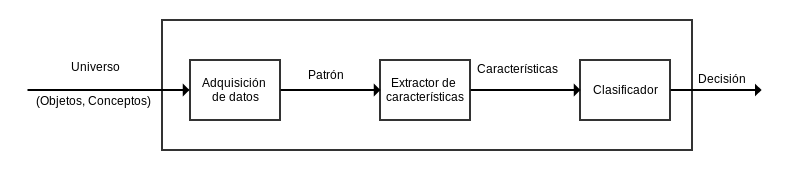
\includegraphics[width=1\textwidth]{Figuras/Diagramas/estado_del_arte/Reconocimiento_de_patrones.png}
  \caption{Arquitectura básica de un sistema de reconocimiento de patrones.}
  \label{art:fig:arquitectura}
\end{figure}


En este trabajo se define el reconocimiento de patrones como un área de la Inteligencia Artificial (IA o AI, artificial intelligence en inglés) enfocada en la extracción de características de un conjunto de imágenes o vídeos, las cuales definen los patrones que serán utilizados para la creación de un modelo que permita clasificar nuevas entradas. Podemos describir este procedimiento en tres procesos como se puede ver en la Figura~\ref{art:fig:arquitectura}: adquisición de datos, extracción de características y toma de decisiones. 

	\textbf{Adquisición de datos.} La adquisición de datos es el procedimiento encargado de sensar la información del mundo real, para esto se utilizan distintos sensores dependiendo del área al cual se quiera aplicar el PR. Estos sensores tienen distintas respuestas dependiendo de su calidad o las variables del medio ambiente como la luminosidad, ruido ambiental, \etc. Para este trabajo nos enfocaremos en los sensores de imágenes instalados en las cámaras que capturan los vídeos que luego serán clasificados por nuestro sistema.
	
	\textbf{Extracción de características.} La extracción de características es el primer proceso en el cual interviene la maquina, tiene como objetivo transformar las señales adquiridas por la etapa anterior a una representación vectorial capas de ser interpretada por los clasificadores para la toma de decisiones. Este procedimiento es el que mas cambia a la hora de construir sistemas de reconocimiento de patrones, esto debido a que existe una gran variación de la implementación a realizar dependido del problema que se requiera atacar. Para esta etapa existen distintos métodos que se pueden utilizar para resolver el problema propuesto, estos serán mayormente estudiados en la Sección~\ref{sec:type_fe}.
	
	\textbf{Toma de decisiones.} La toma de decisiones es la ultima etapa del PR, esta se encarga de realizar la toma de decisiones utilizando las características extraídas en la etapa anterior. Para esto podemos dividir este bloque en dos sub-procesos, entrenamiento y clasificación. El entrenamiento consiste en tomar una gran cantidad de datos ya clasificados anteriormente de forma correcta por algún experto en el tema, y utilizar estos datos para poder crear un modelo el cual divida el espacio vectorial representado por las características de cada uno de los datos de entrenamiento. La clasificación consiste en utilizar el modelo creado en la etapa de entrenamiento para poder clasificar nuevas entradas no tomadas en cuenta en el entrenamiento. Para la etapa de creación del modelo se pueden utilizar distintas técnicas que permiten dividir el espacio en distintas regiones dependiendo de las etiquetas o clases a las cuales se requiera clasificar, tales como: Redes bayesianas, técnicas de clustering, redes neuronales, Modelos ocultos de Markov (HMM, hidden Markov models en inglés). Para el desarrollo de nuestro método utilizaremos las maquinas de soporte vectorial~\cite{Cortes1995,Hearst1998} (SVM, Support Vector Machines en inglés), las cuales permiten realizar una clasificación de muchas clases en un mismo espacio vectorial al mismo tiempo. 


	\subsection{Support Vector Machines}
	\label{sec:svm}
	Las Máquinas de Vectores de Soportes (SVM por sus siglas en inglés) son herramientas fundamentales en sistemas de aprendizaje automático, se basan en  implementar reglas de decisión complejas, por medio de un kernel que permite mapear los puntos de entrenamiento a un espacio de mayor dimensión, esta técnica es llamada \textit{kernel trick}, y consiste en realizar una transformación del espacio vectorial a analizar, donde se pueda encontrar una recta o hiperplano que permita dividir las muestras en dos grupos, este \textit{kernel trick}, puede ser visualizado en la Figura~\ref{art:fig:kernel_trick}, en donde vemos que por medio de un kernel radial, se logra encontrar una recta que separe las muestras en dos grupos. 
	
	Las máquinas son utilizadas para la clasificación y análisis de regresión permitiendo generar un modelo de predicción dado un conjunto de datos de entrada, y posteriormente utilizar este modelo para clasificar nuevos datos.
	
	\begin{figure}[tb]
		\centering
		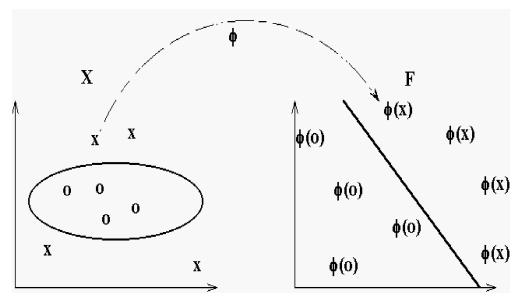
\includegraphics[width=.5\textwidth]{Figuras/Diagramas/estado_del_arte/kernel_trick.jpg}
		\caption{Gráfica demostrativa del cambio en el espacio vectorial al utilizar un kernel.}
		\label{art:fig:kernel_trick}
	\end{figure}
	
	\begin{figure}[t]
		\centering
		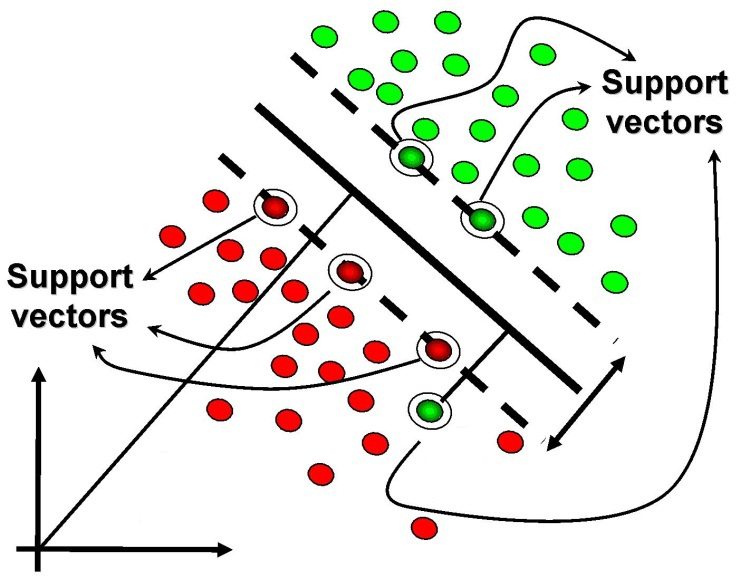
\includegraphics[width=.5\textwidth]{Figuras/Diagramas/estado_del_arte/support_vectors.jpg}
		\caption{Gráfica demostrativa de la elección de los vectores de soporte.}
		\label{art:fig:support_vectors}
	\end{figure}
		
	La idea general de SVM es solucionar un problema de clasificación de dos clases mediante una barrera de decisión, para encontrar esta barrera se realiza la elección de vectores de soporte, los cuales serán los encargados de ayudar a solucionar el problema de optimización, esta elección puede ser vista en la Figura~\ref{art:fig:support_vectors}, donde las muestras encerradas en circulo representa a los vectores de soporte, los cuales ayudan a encontrar la barrera de decisión o hiperplano que separa las muestras en dos grupos, de tal forma que todos los vectores de soporte tienen la misma distancia a dicha barrera. Estos métodos evolucionaron con el tiempo y se utilizan para poder solucionar el problema de clasificación de múltiples clases.

	Existen distintos tipos de Kernels que permiten encontrar hiperplanos mas eficientes dependiendo de la representación de los datos de entrenamiento, algunos de los mas conocidos son:
	
	\textbf{Lineal}: Kernel lineal, no realiza ninguna transformación vectorial, es utilizado cuando las muestras son linealmente separables,
	\begin{equation}
	\kappa(x_i,x_j) = x_{i}^{T}x_j;
	\label{k:lineal}
	\end{equation}
	
	\textbf{RBF}: Kernel radial, es la mejor opción la mayoría de las veces, permite realizar una transformación a un espacio curvo, en el cual una recta o hiperplano de este espacio curvo es representada por circunferencia en el plano cartesiano, en este kernel se tiene una variable de suavizado llamada $\gamma$,
	\begin{equation}
	\kappa(x_i,x_j) = e^{-\gamma||x_i - x_j||^2 }, \gamma > 0;
	\label{k:RBF}
	\end{equation}
	
	\textbf{Poly}: Kernel polinomial, mapea en función del grado del polinomio, en general realiza una transformación a un espacio vectorial, en el cual una recta o hiperplano es representada por un polinomio de grado $degree$ en el plano cartesiano, la variable $coef0$ representa un corrimiento y $\gamma$ el suavizado,
	\begin{equation}
	\kappa(x_i,x_j) = (\gamma x_{i}^{T}x_j + coef0)^{degree}, \gamma > 0;
	\label{k:Poly}
	\end{equation}
	
%	\textbf{Chi-Square}: Kernel basado en la distribución Chi-Square.
%	\begin{equation}
%	\kappa(x_i,x_j) = e^{-\gamma X^{2}(x_i,x_j)}, X^{2}(x_i,x_j) = \frac{(x_i - x_j)^2}{(x_i + x_j)}, \gamma > 0;
%	\label{k:chi-square}
%	\end{equation}
	
	\textbf{Histogram Intersection}: Utilizado para la clasificación de histogramas, es generalmente utilizado cuando las muestras representan histogramas.
	\begin{equation}
	\kappa(x_i,x_j) = \min(x_i,x_j).
	\label{k:Inter}
	\end{equation}


Para efectos de este trabajo, SVM es utilizado para poder generar el modelo final que permita clasificar las seis expresiones faciales canónicas, utilizando los descriptores obtenidos luego de la extracción de características.

\section{Reconocimiento de expresiones faciales}
\label{sec:fer}
Las expresiones faciales constituyen una guía básica en la interacción social. Por ello, las alteraciones en su expresión o reconocimiento suponen una importante limitación para la comunicación. Ya que las expresiones del rostro son la variable que más se observa para obtener información de las emociones de nuestros interlocutores; si bien es cierto que tenemos un elevado control sobre nuestra expresividad facial, diversos estudios han demostrado que, cuando una persona está utilizando una expresión facial no acorde con su verdadero estado de ánimo, en su cara aparecen durante breves momentos señales de la expresión verdadera que a menudo pasan desapercibidas por las demás personas, estas se conocen como expresiones faciales universales.


\subsection{Expresiones faciales universales}
\label{sec:type_fe}

Las expresiones faciales del rostro humano tienen una infinidad de posibles variaciones que permiten la comunicación, regulación y adecuación de las emociones en el contexto social.

Darwin afirma en uno de  sus estudios publicado a fines del siglo XIX, que nosotros no podemos entender las expresiones emocionales humanas sin entender las expresiones emocionales de los animales, para esto, él argumenta que nuestras expresiones son determinadas en gran parte por nuestra evolución~\cite{Darwin1956,Darwin1998}. En la actualidad Paul Ekman, psicólogo pionero en el estudio de las emociones y su relación con la expresión facial, propone que las expresiones faciales están compuestas por micro-expresiones muy breves, que duran sólo una fracción de segundo. Estas se producen cuando una persona ya sea deliberadamente o inconscientemente esconde un sentimiento~\cite{Ekman1981}.

\newpage
Ekman y Friesen definen que existen seis expresiones universales~\cite{Ekman2003}: 

\begin{enumerate}
	\item Alegría (Happiness): se produce mediante la contracción del músculo que va del pómulo al labio superior y del orbicular que rodea al ojo. También se elevan las mejillas. 
	\item Asco (Disgust): Existe una ligera contracción del músculo que frunce la nariz y estrecha los ojos. El gesto de la nariz arrugada es simultáneo al de la elevación del labio superior. 
	\item Ira (Anger): Se produce con una mirada fija, cejas juntas y hacia abajo, y existe una tendencia a apretar los dientes. 
	\item Miedo (Fear): Se observa los párpados superiores elevados al máximo e inferiores tensos. Las cejas levantadas se acercan y los labios se alargan hacia atrás. 
	\item Sorpresa (Surprise): Los párpados superiores suben, pero los inferiores no están tensos, la mandíbula suele caer. 
	\item Tristeza (Sadness): Se manifiesta cuando los párpados superiores caen y las cejas se angulan hacia arriba. El entrecejo se arruga y los labios se estiran de forma horizontal.
\end{enumerate}


\subsection{Métodos de reconocimiento de expresiones faciales}
Los Métodos de reconocimiento de expresiones faciales pueden ser divididos en dos grupos: métodos geométricos y métodos de apariencia, los geométricos consisten en extraer características de la geometría del rostro, por el contrario, los métodos de apariencia se encargan de extraer características de las texturas de la imagen y encontrar patrones ocultos. Para mas información acerca de los métodos de reconocimiento de expresiones faciales  ver otros estudios como los realizados por Pantic~y~Rothkrantz~\cite{Pantic2000} o Zeng~\etal~\cite{Zeng2009}. A su vez cada uno de estos grupos tiene métodos que ayudan a reconocer las expresiones en imágenes o en vídeos. Para esta investigación nos centramos en estudiar solo los métodos basados en apariencia.

\subsubsection{Métodos basados en características geométricas}
\label{sec:met_geo}
Los métodos geométricos se basan en detectar formas y regiones de la cara que se esta procesando, así como puntos de características faciales (\eg ojos, comisuras de la boca, \etc). 
Luego de encontrar las regiones importantes del rostro que se está analizando se procede a realizar la clasificación. Los métodos geométricos al ser aplicados sobre imágenes dinámicas o vídeos, realizan el procedimiento de encontrar cada una de estas regiones importantes del rostro que aportan la mayor cantidad de información, y luego se realiza el seguimiento a lo largo de la secuencia de cuadros del vídeo. Una de las grandes ventajas de estos métodos, es que al ser enfocado en encontrar una cantidad determinada de puntos, son algoritmos muy rápidos y de fácil aplicación a sistemas de reconocimiento en tiempo real. A su vez no son tan robustos como los basados en apariencia.


\subsubsection{Métodos basados en características de apariencia}
\label{sec:met_apa}
Se basan en detectar los movimientos de las texturas en la imagen, en el caso de imágenes con rostros humanos, cambios o deformaciones en la piel (\eg arrugas, protuberancias, surcos, \etc). En si son métodos que no se basan en encontrar ciertos puntos específicos del rostro, sino que encuentran regiones importantes de las texturas a analizar. Existen distintas aplicaciones de estos métodos, tanto sobre imágenes estáticas como para vídeo o imágenes dinámicas.  

	\subsubsection{Métodos basados en características sobre imágenes}
	\label{sec:met_imagen}
		Son métodos enfocados en encontrar ciertas regularidades existentes entre las texturas de la imagen a analizar, ejemplos:

		\subsubsection{Local Binary Patterns}
		\label{sec:lbp}
		Método introducido por Wang y He~\cite{Wang1990}, consiste en realizar una codificación del píxel de interés con respecto a los valores de sus vecinos. En simples palabras se realiza un proceso de máscara en el cual se restan los píxeles del vecindario con el píxel central, si la resta es negativa o cero se asigna un cero en la posición del vecino, por el contrario si es positiva se asigna un uno. Luego de esto, se realiza una concatenación de los vecinos y se obtiene un código binario que es transformado a base 10. Dicho número es asignado como nuevo valor del píxel visitado~\cite{Ojala1994,Ojala2002,Ahonen2004,Shan2009}. Este procedimiento puede ser visto en la Figura~\ref{art:fig:lbp}.
		
\begin{figure}[tb]
  \centering
   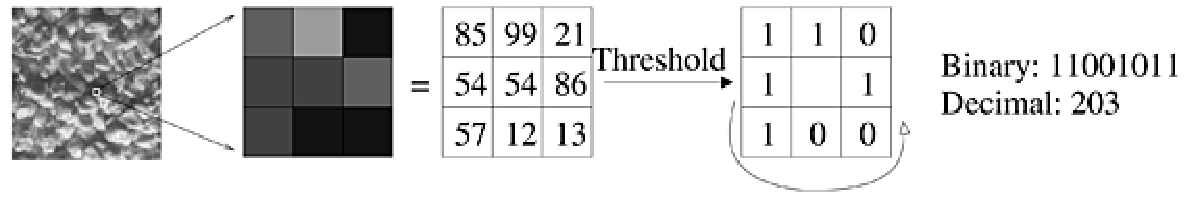
\includegraphics[width=1\textwidth]{Figuras/lbp.pdf}
  \caption{Proceso de codificación de LBP~\cite{Ahonen2006}.}
  \label{art:fig:lbp}
\end{figure}

Luego de realizar el proceso en todos los pixeles de la imagen se procede a realizar un histograma de los nuevos valores, este histograma es el descriptor de la imagen, el cual es utilizado para entrenar los modelos o simplemente ser clasificado.

Otros métodos que utilizan LBP antes de la obtención del descriptor dividen la imagen en $n$ secciones de igual o distintas áreas, y realizan el cálculo del histograma para cada una de estas secciones. Luego concatenan cada uno de los histogramas en un orden específico y se obtiene un macro descriptor más detallado de la imagen~\cite{Ahonen2006}.

		\subsubsection{Local Directional Number Pattern}
		\label{sec:ldn}
		Método introducido por Ramírez \etal~\cite{RamirezRivera2013}, consiste en realizar una codificación de los píxeles utilizando toda la vecindad. Utiliza el operador de Kirsch~\cite{Kirsch1971}, el cual permite encontrar las gradientes o bordes de la imagen las ocho direcciones. El método realiza un proceso de máscara para cada uno de los detectores de bordes de Kirsch, luego para cada píxel a codificar se obtiene el índice de la mascara que obtuvo la mayor intensidad al ser aplicada, a su vez también se obtiene el índice de la mascara que obtuvo el menor valor. Luego estos índices son transformados a una base binaria de tres dígitos y concatenados obteniendo una cadena binaria de seis dígitos, esta es nuevamente transformada a decimal y este valor decimal (entre $0$ y $63$) es el nuevo valor que representa el píxel, este proceso puede ser visto en la Figura~\ref{art:fig:ldn}, donde en la parte izquierda de la imagen podemos ver el proceso de aplicación de las ocho mascaras de Kirsch a la imagen, luego para cada pixel a codificar se escogen el mayor y menor valor resultante en las mascaras, los cuales con concatenados y el resultado es la codificación del píxel o nuevo valor resultante.
		
\begin{figure}[tb]
  \centering
   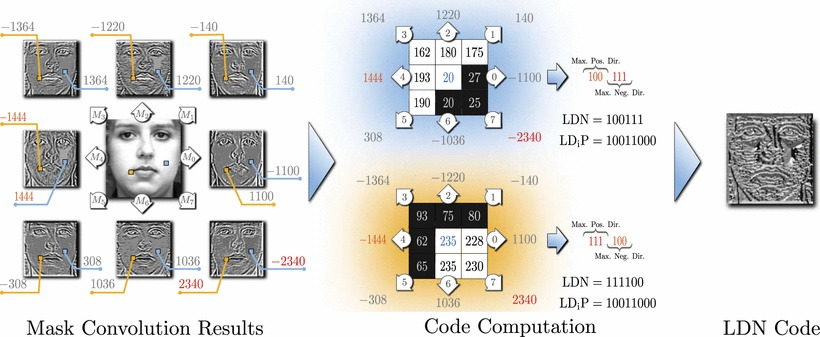
\includegraphics[width=1\textwidth]{Figuras/ldn.jpg}
  \caption{Proceso de codificación de LDN~\cite{RamirezRivera2013}.}
  \label{art:fig:ldn}
\end{figure}

		Luego de codificar toda la imagen, se realiza un histograma de la imagen, este es utilizado como descriptor para la posterior clasificación. También la imagen puede ser segmentada por una grilla, en la cual se calcula un histograma para cada una de las grillas, y luego se concatenan en un orden específico.

	\subsubsection{Métodos basados en características sobre imágenes dinámicas o videos}	
	\label{sec:met_videos}
	Para estos métodos se introduce la variable temporal $t$, la cual es la encargada de regir el movimiento de los píxeles a lo largo del tiempo, al igual que los métodos sobre imágenes estáticas, estos métodos resuelven el problema planteado de forma similar, pero adaptando las técnicas a la nueva variable.

		\subsubsection{Volume Local Binary Patterns.}
		\label{sec:vlbp}
		Método introducido por Zhao y Pietikäinen~\cite{Zhao2006,Zhao2007a,Zhao2007}, basado en LBP para imágenes dinámicas, el cual se basa en tres variables: $L$ la cantidad de cuadros que entran en la creación del patrón, $P$ el tamaño del vecindario a seleccionar y $R$ el radio del cual se escogen los vecinos. 
El método VLBP consiste en realizar una codificación basada en LBP, ahora incluyendo la variable temporal $L$ que indica desde qué cuadro se comienza a realizar la resta del píxel seleccionado con el central.
Éste es un proceso muy costoso debido a que mientras mayor sea la cantidad de vecinos a seleccionar, mayor será la cantidad de dígitos binarios, lo cual implica un mayor espectro de números resultantes en la codificación. Este proceso puede ser visto en la Figura~\ref{art:fig:vlbp}.

\begin{figure}[tb]
  \centering
   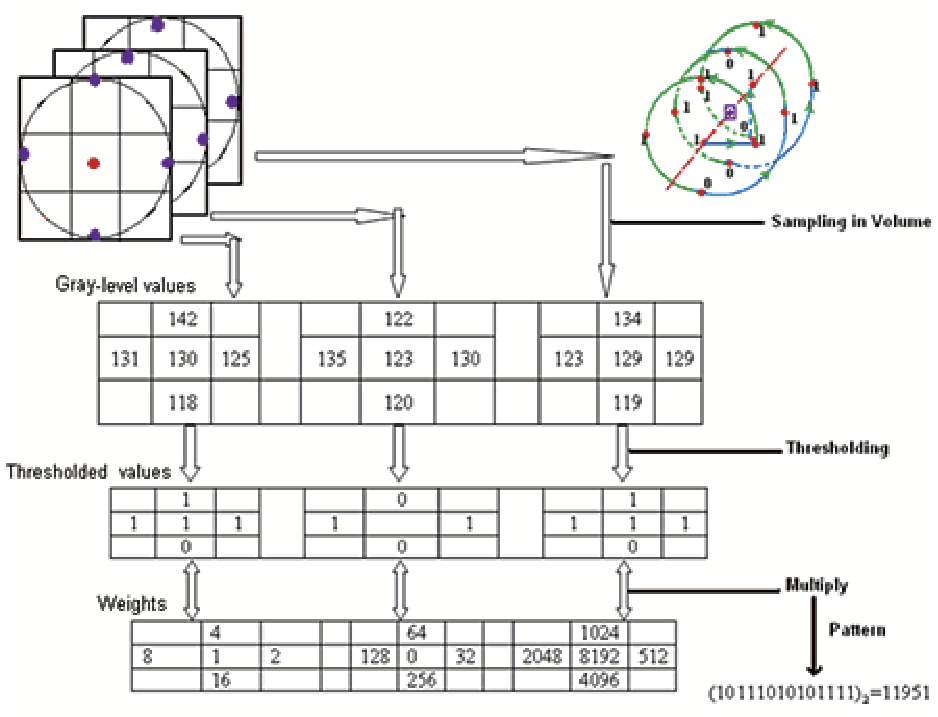
\includegraphics[width=0.7\textwidth]{Figuras/vlbp.pdf}
  \caption{Proceso de codificación de VLBP utilizando $L$~=~1, $P$~=~4 y $R$~=~1~\cite{Zhao2007}.}
  \label{art:fig:vlbp}
\end{figure}


		\subsubsection{Local Binary Patterns-Three Ortogonal Planes}
		\label{sec:lbp-top}
		 Es un método basado en LBP para imágenes dinámicas, consiste en crear tres planos ortogonales que se intersectan en el píxel de interés, siendo estos el plano $XY$, $XT$, y $YT$ (cuadro actual, movimiento temporal en $X$ y en $Y$ respectivamente). 

Para poder obtener el patrón de la imagen se realiza el mismo proceso de resta con los píxeles del vecindario seleccionado, pero a diferencia de los métodos estáticos que solo se realizan en el plano $XY$, este también se realiza para los planos $XT$ e $YT$.\@ Con esto se obtiene un histograma para cada plano, los cuales son concatenados y forman el macro descriptor de la imagen~\cite{Zhao2007}. Este proceso puede ser visto en la Figura~\ref{art:fig:lbptop}.


\begin{figure}[tb]
  \centering
   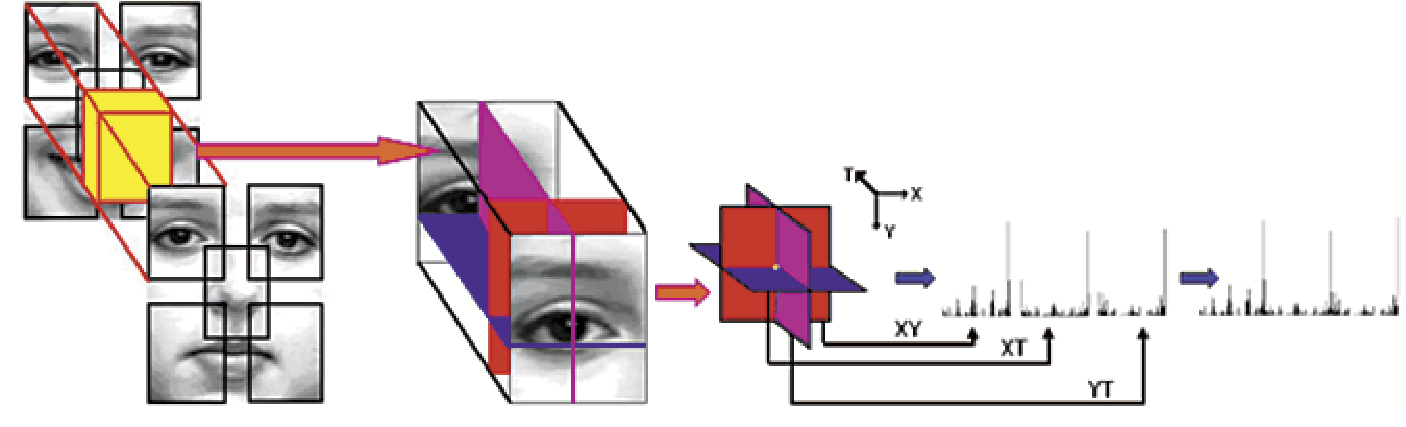
\includegraphics[width=1\textwidth]{Figuras/lbptop.pdf}
  \caption{Proceso de codificación de LBP-TOP~\cite{Zhao2007}.}
  \label{art:fig:lbptop}
\end{figure}


\section{Reconocimiento y corrección de rostros}
\label{sec:rec_rostros}

	\subsection{Framework Viola-Jones}
	\label{sec:viola-jones}
	Introducido por Viola y Jones~\cite{Jones2003}, es un método que utiliza clasificación en cascada, y un entrenador de clasificadores débiles basado en AdaBoost~\cite{Freund1995}. Este algoritmo consiste en subdividir la imagen a analizar en pequeñas sub-imágenes, las cuales son entregadas a una serie de clasificadores débiles (etapas), cada uno con un conjunto de características visuales. El método consiste en que cada sub-imagen es evaluada por los clasificadores débiles de la cascada, si en una es encontrado un rostro, esta sub-imagen es entregada al siguiente clasificador, el cual revisa de forma mas rigurosa la imagen. Si la imagen es aceptada por todos los clasificadores, esta es clasificada como un rostro.
	
	\subsection{Corrección de movimiento rígido}
	\label{sec:rigid}
	Los métodos de corrección de movimiento rígido consisten en utilizar técnicas de rotación y traslación de regiones de la imagen, esto para poder ajustar el movimiento de todos los cuadros del video sobre una región especifica. Este tipo de corrección no alteran el tamaño de la imagen, sólo su ubicación y el ángulo su rotación.


\section{Bag of Visual Words}
\label{sec:bag_of_words}
\textit{Bag of visual words}, es una técnica utilizada para la clasificación de documentos, consiste en la creación de un descriptor de cada documento a partir de la frecuencia de aparición de cada una de las palabras que este en la bolsa. Esta bolsa es construida como un diccionario que contiene todas las palabras que aparecen en los documentos a clasificar.

Recientemente esta técnica también es utilizada para la clasificación de imágenes y es conocida como Bag of Visual Words. Para poder utilizar la misma teoría, las palabras son reemplazadas por características extraídas de las imágenes. El problema es que la cantidad de características es muy alta y con una muy baja probabilidad de ser iguales entre ellas, por lo cual es necesario agrupar en conjuntos de características, las cuales son utilizados para construir los descriptores de las imágenes. Estos conjuntos de características son representados por un vector o centroide, el cual es el representante del grupo, luego de esto se procede a construir la bolsa de palabras agrupando todos estos centros como el vocabulario visual de las imágenes. Para poder encontrar los centroides de cada uno de los grupos es necesario utilizar técnicas de agrupamiento o \textit{clustering} como $k$-means. Implementaciones de esta técnica en clasificación de imágenes pueden ser vistas en distintas investigaciones~\cite{Csurka2004,Dollar2005,Sivic2009}.

	\subsection{$K$-means}
	\label{sec:k-means}
	$K$-means es un método introducido por Lloyd~\cite{Lloyd1982} utilizado mayormente en minería de datos, tiene como objetivo principal realizar una partición sobre un conjunto de datos en $k$ grupos, donde cada dato pertenece a solo un grupo.
	El algoritmo consiste en encontrar los centroides o \textit{clusters} de los $k$ grupos que se requiere crear, esto se realiza con un proceso iterativo, el cual dada la elección inicial de los centroides, calcula la distancia a cada uno de los datos, de tal forma que cada dato es introducido en un grupo. Luego recalcula el centroide de cada grupo como la media de cada uno de los datos que pertenecen a ese \textit{cluster}. Esto se realiza hasta cumplir con los requerimientos de parada, los cuales pueden ser: la inexistencia de nuevas asignaciones de grupo, pequeños cambios en los centroides o cambios mínimos en la suma del error cuadrático.
	Uno de los grandes problemas de este algoritmo, es la elección de los centroides iniciales, esto debido a que cada instancia puede encontrar distintos máximos locales, por lo cual esto se puede solucionar de forma que se corren distintas instancias con los mismos datos, y luego se calcula un promedio para cada uno de los $k$ centros.
	Otro de los grandes problemas de este método es la elección de la métrica de distancia a utilizar, ya que dependiendo de el tipo de los vectores a utilizar existen distintas formas de calcular la distancia, lo cual cambia los resultados de los resultados.
			
	%\subsubsection{Métricas de distancia}
	%\label{sec:matricas_de_distancia}
	%Las métricas de distancia se utilizan para saber que tan cerca o lejos esta un vector de otro, por lo cual esto permite poder tener la distancia entre dos vectores pertenecientes al mismo espacio vectorial. 
	%Sean dos vectores $p$-dimensionales $x$,$y$ de un subespacio de $\mathds{R}^p$. Entonces, se pueden definir las siguientes medidas de distancia entre $x$ e $y$~\cite{Pereira2010}:
	
%\paragraph{Distancia Euclidiana}\label{deuclidiana}

%\begin{equation}
%d(x,y) = \Big\{\sum_{i} (x_i-y_i)^2\Big\}^{1/2}
%\end{equation}


%\paragraph{Distancia Euclidiana %cuadrada}\label{deuclidianacuad}

%\begin{equation}
%d(x,y) = \sum_{i} (x_i-y_i)^2
%\end{equation}


%\paragraph{Distancia de Manhattan}\label{dmanhattan}

%\begin{equation}
%d(x,y) = \sum_{i} \vert x_i-y_i\vert
%\end{equation}

%\paragraph{Distancia de Minkowski}\label{dminkowski}

%\begin{equation}
%d(x,y) =\Big\{ \sum_{i} \vert x_i-y_i\vert^{1/l}\Big\}^l
%\end{equation}


%\paragraph{Distancia de potencia}\label{dpotencia}

%\begin{equation}
%d(x,y) = \Big\{\sum_{i} (x_i-y_i)^p\Big\}^{1/r}
%\end{equation}

%\paragraph{Distancia del coseno}\label{dcoseno}

%\begin{equation}
%d(x,y) = \frac{\sum_{i} (x_iy_i)}{\sqrt{\sum_{i} %x_i^2}\sqrt{\sum_{i} y_i^2}}
%\end{equation}


%\paragraph{Correlaci\'on de Pearson}\label{dpearson}

%\begin{equation}
%d(x,y) = \frac{\sum_{i} %(x_i-\bar{x})(y_i-\bar{y})}{\sqrt{\sum_{i} %(x_i-\bar{x})^2}\sqrt{\sum_{i} (y_i-\bar{y})^2}}
%\end{equation}
